\documentclass[conference]{IEEEtran}

\newcommand{\thetitle}{Non-Parametric Discrete Mixture Model Recovery via Nonnegative Matrix Factorization}

%!TEX root = paper.tex

\usepackage[labelfont=bf,small]{caption}
\usepackage[font=small,labelfont=bf,position=top,nearskip=0em]{subfig}
\usepackage{cite,amsmath,amssymb,rotating,multirow,bigstrut,url,wrapfig,relsize,paralist,array,mathtools,units}
\usepackage[hyperfigures,bookmarks,bookmarksopen,bookmarksnumbered,colorlinks,linkcolor=black,citecolor=black,filecolor=blue,menucolor=black,pagecolor=blue,frenchlinks=true,pdftitle={\thetitle}]{hyperref}

%!TEX root = paper.tex

%% LABELING COMMANDS
\renewcommand{\sec}[1]{\label{sec:#1}}
\newcommand{\eqn}[1]{\label{eqn:#1}}
\newcommand{\fig}[1]{\label{fig:#1}}
\newcommand{\tab}[1]{\label{tab:#1}}
\newcommand{\thm}[1]{\label{thm:#1}}
\newcommand{\defn}[1]{\label{def:#1}}

%% REFERENCING COMMANDS
\newcommand{\Appendix}[1]{\hyperref[sec:#1]{Appendix~\ref*{sec:#1}}}
\newcommand{\Section}[1]{\hyperref[sec:#1]{Section~\ref*{sec:#1}}}
\newcommand{\Equation}[1]{\hyperref[eqn:#1]{Equation~\ref*{eqn:#1}}}
\newcommand{\Figure}[1]{\hyperref[fig:#1]{Figure~\ref*{fig:#1}}}
\newcommand{\Table}[1]{\hyperref[tab:#1]{Table~\ref*{tab:#1}}}
\newcommand{\Theorem}[1]{\hyperref[thm:#1]{Theorem~\ref*{thm:#1}}}
\newcommand{\Definition}[1]{\hyperref[def:#1]{Definition~\ref*{def:#1}}}

%% MATHEMATICAL NOTATIONS

% common algebraic domains
\newcommand{\N}{\mathbb{N}}
\newcommand{\Z}{\mathbb{Z}}
\newcommand{\Q}{\mathbb{Q}}
\newcommand{\R}{\mathbb{R}}

% standard operators & functors
\renewcommand{\Pr}{\mathrm{Pr}}
\newcommand{\Image}{\text{Im}}
\newcommand{\Kernel}{\text{Ker}}

% common constructs
\newcommand{\abs}[1]{{\left|#1\right|}}
\newcommand{\absx}[1]{{|#1|}}
\newcommand{\card}[1]{{\left|#1\right|}}
\newcommand{\cardx}[1]{{|#1|}}
\newcommand{\norm}[1]{{\lVert#1\rVert}}
\newcommand{\normx}[1]{{\Vert#1\Vert}}
\newcommand{\set}[1]{{\left\{#1\right\}}}
\newcommand{\setx}[1]{{\{#1\}}}
\newcommand{\parens}[1]{{\left(#1\right)}}
\newcommand{\parensx}[1]{{(#1)}}
\newcommand{\bracket}[1]{{\left[#1\right]}}
\newcommand{\bracketx}[1]{{[#1]}}
\newcommand{\seq}[1]{{\left<#1\right>}}
\newcommand{\seqx}[1]{{\lvert#1\rvert}}
\newcommand{\tuple}[1]{{\left<#1\right>}}
\newcommand{\tuplex}[1]{{\lvert#1\rvert}}
\newcommand{\floor}[1]{{\left\lfloor#1\right\rfloor}}
\newcommand{\floorx}[1]{{\lfloor#1\rfloor}}
\newcommand{\ceil}[1]{{\left\lceil#1\right\rceil}}
\newcommand{\ceilx}[1]{{\lceil#1\rceil}}
\newcommand{\round}[1]{{\left[#1\right]}}
\newcommand{\roundx}[1]{{[#1]}}
\newcommand{\fracx}[2]{{#1/#2}}
\newcommand{\fracp}[2]{{\left(\frac{#1}{#2}\right)}}
\newcommand{\fracpx}[2]{{(#1/#2)}}
\newcommand{\smallfrac}[2]{{\textstyle{\frac{#1}{#2}}}}

% standard notations
\newcommand{\trans}[1]{{#1}^T}
\newcommand{\inner}[2]{{#1}\trans{#2}}
\newcommand{\cross}{\times}
\newcommand{\tensor}{\otimes}
\newcommand{\directsum}{\oplus}
\newcommand{\iso}{\cong}
\newcommand{\union}{\cup}
\newcommand{\inter}{\cap}
\newcommand{\Union}{\bigcup}
\newcommand{\Inter}{\bigcap}
\newcommand{\conj}{\wedge}
\newcommand{\disj}{\vee}
\newcommand{\Conj}{\bigwedge}
\newcommand{\Disj}{\bigvee}
\newcommand{\defeq}{=}
\renewcommand{\emptyset}{\varnothing}
\renewcommand{\setminus}{\,\raisebox{1pt}{$\smallsetminus$}\,}
\newcommand{\eldiv}{\,./\,}
\newcommand{\diag}{\text{diag}}
\newcommand{\rStoch}{\text{rs}}

%% FORMATTING BEHAVIORS
\newcommand{\caps}[1]{{\smaller{#1}}}
\newcommand{\latin}[1]{\textit{#1}}
\newcommand{\defterm}[1]{\textit{#1}}
\newcommand{\newfootnote}[2]{\newcommand{#1}{\footnote{#2} }}
\renewcommand{\bullet}{\raisebox{2pt}{$\centerdot$}}
\renewcommand{\arraystretch}{1.3}


\title{\vspace{-0.25em}\thetitle}
\author{
{\large{Stefan~Karpinski, John~R.~Gilbert, Elizabeth~M.~Belding}} \vspace{0.25em}\\
Department of Computer Science \\
University of California, Santa Barbara \vspace{0.35em}\\
\textit{\{sgk,gilbert,ebelding\}@cs.ucsb.edu}
}

\bibliographystyle{IEEEtran}

\newcommand{\figurename}{Figure}
\newcommand{\tablename}{Table}

\begin{document}
\maketitle

Mixture modeling expresses probability densities as convex combinations of constituent probability distributions:
\begin{align}\eqn{mixture-model}
  q_i(x) = \sum_{j=1}^r w_{ij} p_j(x),
\end{align}
Here $q_i$ and $p_j$ are density functions, and $w_{ij}$ are nonnegative weights, summing to unity for each $i$.
In classical mixture modeling, the constituent density functions, $p_j$, are assumed to be from some class of parametric distributions.
Various well established algorithms, using expectation minimization (\caps{EM}), can optimally recover the weights, $w_{ij}$, given an observed sample of values from $q_i$~\cite{MMEM}.

In certain settings, however, mixture modeling is desirable, but the constituent distributions are neither known in advance, nor can they be assumed to be parametric.
In this work, we demonstrate how, for discrete event spaces, nonnegative matrix factorization (\caps{NMF}) can be effectively used to simultaneously recover both weights and constituent distributions, given a large collection of variably-sized samples from mixtures.
% Our work addresses mixture models over discrete event spaces, but can be applied readily to continuous spaces, since continuous quantities can be discretized, and our techniques then applied to the resulting large discrete spaces. Since our approach makes no parametric assumptions, the results are no less valid.

For discrete event spaces, \Equation{mixture-model} is expressed succinctly as matrix multiplication.
Letting $Q_{ik} = q_i(k)$, $W_{ij} = w_{ij}$, and $P_{jk} = p_j(k)$ we have:
\begin{align}\eqn{mixture-model-matrix}
  Q = WP.
\end{align}
% The matrices are all be row-stochastic.
The problem of inferring both the weights, $w_{ij}$, and constituent distributions, $p_j$, from a collection of mixtures, $q_i$, is equivalent to finding the factors $W$ and $P$ given $Q$.
All three matrices are constrined to be row-stochastic, meaning that all entries are nonnegative, with rows summing to unity.

The problem of finding such a factorization is known as nonnegative matrix factorization.
Such factorizations are not unique, so perfect recovery of $W$ and $P$ cannot generally be achieved.
On the other hand, any exact factorization of $Q$, is an equally valid mixture model for the given data.
Since a variety of \caps{NMF} algorithms have been proposed, this problem is partially solved.
Several difficulties remain, however:
\begin{enumerate}
  \item \caps{NMF} is known to be \caps{NP}-hard; thus, all efficient algorithms are heuristic, and may not yield adequate results;
  \item $Q$ is not known exactly, only a finite sample for each distribution row of $Q$ is observed;
  \item The samples for the rows may not have uniform size.
\end{enumerate}
This list is not exhaustive, and we will address and discuss other challenges as well.

Our motivating application is mixture modeling for traces of network flows, whose distributions of packet sizes and inter-packet intervals seem to be effectively modeled as discretized mixture models, using \caps{NMF}~\cite{Karpinski08}.
In this setting, there are several particularly challenging aspects:
\begin{enumerate}
  \item The distribution of sample sizes is heavy-tailed, having a few very large samples, and many very small samples;
  \item The constituent distributions are not uniformly represented: the most prevalent distribution has much larger average weights than the next, and so on.
\end{enumerate}
We will demonstrate using simulated data why both of these properties make factor recovery particularly difficult.

\begin{figure}[b]
\fig{synthetic-basis}
\begin{center}
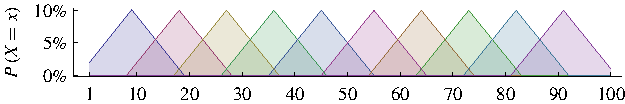
\includegraphics[width=3.5in]{synth/test}
\end{center}
\vspace{-0.7em}
\caption{Discrete distributions used to generate synthetic mixtures.}
\vspace{-0.5em}
\end{figure}

\begin{figure}[b]
\fig{synthetic-weights}
\begin{center}
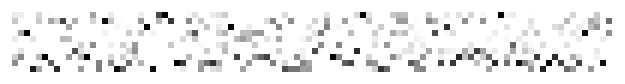
\includegraphics[width=3.5in]{synth/weights}
\end{center}
\vspace{-0.7em}
\caption{Transposed matrix plot of 100 sample weight vectors.}
\vspace{-0.3em}
\end{figure}

To evaluate the effectiveness of \caps{NMF} techniques for discrete mixture model recovery, we use synthetic data, since otherwise the true factors are unknown.
To generate synthetic data, we use saw-tooth patterns as constituent distributions, densities of which are shown in Figure~1.
These distributions are visually distinctive and not well-approximated by standard parametric distributions.
The Pareto distribution is the classic heavy-tailed distribution, and has been shown to describe the distribution of flow sizes in several network trace studies.
Accordingly, we choose sample sizes for each synthetic mixture from a Pareto distribution.
Our synthetic weight matrices are also generated such that the prevalences of the component distributions\,---\,i.e. the column sums of $W$---\,are Pareto-distributed. Figure 2 is a matrix plot of sample rows of randomly generated weights.
% (transposed to save space).

\begin{figure}[t]
\begin{center}
\subfloat[Lee \& Seung, Euclidean Algorithm]
{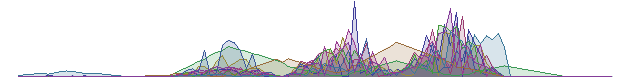
\includegraphics[width=3.5in]{synth/Q_euclidean}}
\subfloat[Lee \& Seung, Kullback-Leibler Algorithm]
{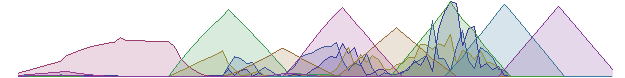
\includegraphics[width=3.5in]{synth/Q_divergence}}
\subfloat[Kim \& Park, ANLS Algorithm]
{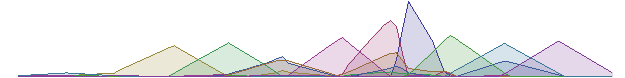
\includegraphics[width=3.5in]{synth/Q_anls}}
\end{center}
\caption{Recovered $P_*$ distributions for standard \caps{NMF} algorithms, with random initialization and perfect knowledge of $Q$.}
\end{figure}

\begin{figure}[t]
\begin{center}
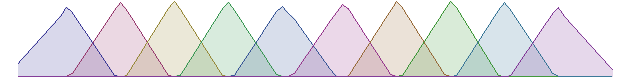
\includegraphics[width=3.5in]{synth/Q_ki}
\end{center}
\vspace{-0.7em}
\caption{$P_0$ computed using SVD/$k$-means initialization.}
\vspace{-1em}
\end{figure}

In short, we find that none of the existing \caps{NMF} algorithms can accurately recover the constituent distributions used to generate synthetic mixtures.
Recovered $P_*$ distributions for Lee and Seung's algorithms~\cite{Lee01}, and Kim and Park's alternating nonnegative least squares (\caps{ANLS}) algorithm~\cite{Kim08} are shown in Figure~3, dramatically illustrating their failure to accurately recover the original distributions.
It is well known that these algorithms may not converge to a globally optimum factorization.
The quality of the end result is largely dependent on the matrices used to initialize the algorithms, which typically are random nonnegative matrices.
To find a better factorization, we use a variation of the most promising initialization technique proposed by Langville~et~al.~\cite{Langville07}:
\begin{enumerate}
  \item Let $Q=USV'$, the singular value decomposition (\caps{SVD}),
  \item Use $k$-means to find $r$ clusters of columns in $V$,
  \item Let $W_0$ be corresponding column centroids in $Q$,
  \item Let $P_0$ be nonnegative minimizing $\norm{Q - W_0 P_0}_F$.
\end{enumerate}
Figure~4 shows that even without any further refinement, this initialization technique already recovers the overall shape of $P$ remarkably well.
Although this recovery appears visually close to optimal, there are differences in shape which limit the quality of the approximation $W_0 P_0$.
Intuitively, this initialization sits on a ridge above a deep valley, where the perfect recovery lies.
If care is not taken, however, the \caps{NMF} algorithms may descend the wrong side of the ridge, moving away from the optimal recovery rather than toward it.
This is precisely what happens when any of these algorithms are applied to $W_0,P_0$ alone, as is shown in Figure~5.

\begin{figure}[t]
\begin{center}
\subfloat[Lee \& Seung, Euclidean Algorithm]
{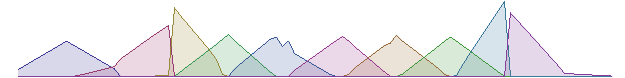
\includegraphics[width=3.5in]{synth/Q_euclidean_ki}}
\subfloat[Lee \& Seung, Kullback-Leibler Algorithm]
{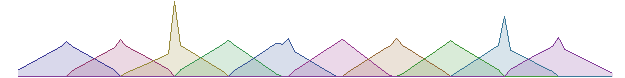
\includegraphics[width=3.5in]{synth/Q_divergence_ki}}
\subfloat[Kim \& Park, ANLS Algorithm]
{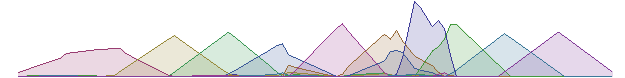
\includegraphics[width=3.5in]{synth/Q_anls_ki}}
\end{center}
\caption{Recovered $P_*$ distributions for standard \caps{NMF} algorithms, with \caps{SVD}/$k$-means initialization and perfect knowledge of $Q$.}
\end{figure}

% \begin{figure}[t]
% \begin{center}
% 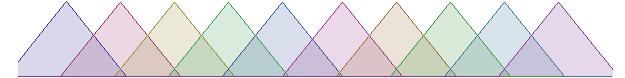
\includegraphics[width=3.5in]{synth/Q_nmf}
% \end{center}
% \vspace{-0.7em}
% \caption{Perfect recovery of $P_*$ using our meta-algorithm.}
% \vspace{-1em}
% \end{figure}

Through a combination of intuition and trial and error, we have found that applying the \caps{ANLS} algorithm for a few dozens of iterations, followed by the Kullback-Leibler algorithm, followed finally by the Euclidean algorithm results in perfect recovery, with error limited only by how many iterations of the Euclidean algorithm one is willing to wait for.
% The recovery result of this meta-algorithm are shown in Figure~6.

The above results all assume perfect knowledge of $Q$.
In real situations, where discrete mixture models must be recovered from experimental data, there is highly imperfect knowledge of $Q$.
Only a finite sample of values from each $q_i$ distribution are observed.
These samples may be of different sizes, and in many situations, the vast majority of the samples are very small, many even consisting of only a single value.
Can the basis matrix, $P$, still be recovered under such circumstances?
Our meta-algorithm can accurately recover $P$, when applied to appropriate estimates of $Q$.

The simplest estimate of $Q$ is based on the sample histogram matrix, $H$:
$H_{ik}$ is the number times the value $k$ was sampled from the distribution $q_i$.
We can approximate $Q$ by the row-stochasticized version of $H$, where each row is divided by its sum;
call this matrix $C$.
If nothing else was known about $Q$, we could not do much better than this approximation.
We know, however, that $Q$ has rank $r$:
we can use \caps{SVD} to find the best rank $r$ approximation of $H$.
Why use the \caps{SVD} approximation of $H$ rather than of $C$?
By applying the \caps{SVD} to $H$, we are giving each row weight proportional to its sample size in computing our approximation, thus giving more weight to more precisely known rows.
The \caps{SVD} approximation matrix may have negative values, since we know $Q$ has none, we force these to be zero.\footnote{This may cause the approximation to become no longer rank $r$. It will, however, remain nearly rank $r$, in the sense that it will have $r$ large singular values and the rest much smaller.}
Let this nonnegative, nearly rank $r$ approximation of $H$ be $A$ and $R$ its row-stochastization.

To successfully apply our meta-algorithm to sampled data, the steps must be applied as follows:
\begin{enumerate}
  \item Compute $W_0,P_0$ from \caps{SVD}/$k$-means on $R$.
  \item Iterate \caps{ANLS} on $R$ starting with $W_0,P_0$.
  \item Let $W_*$ be nonnegative minimizing $\norm{H - W_* P_*}_F$. 
  \item Iterate Kullback-Leibler on $H$ starting with $W_*,P_*$.
  \item Iterate Euclidean on $H$ starting with $W_*,P_*$.
\end{enumerate}
This meta-algorithm can recover $P$ very well, even when $Q$ is sampled with infinite variance, and when the prevalences of constituent distributions follow a power law. Accurate recovery from sampled data is shown in Figure~6.

\begin{figure}[t]
\begin{center}
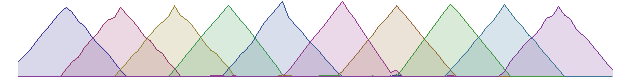
\includegraphics[width=3.5in]{synth/S_nmf}
\end{center}
\vspace{-0.7em}
\caption{Accurate recovery of $P_*$ from sampled data.}
\vspace{-1em}
\end{figure}

% Intuitively, since the sum of each row of $H$ is equal to its sample size, that row's weight in determining the best approximation is proportional to its sample size.
% Therefore, we want to do our approximation giving more weight to rows with more data.



% Unfortunately, 
% Moreover, the error of the estimate does not follow the typical model of a noise matrix added to $Q$.
% 
% 
% Can the basis matrix, $P$, still be recovered under such circumstances?
% 
% In fact, the meta-algorithm described above does recover $P$ quite well, so long as care is taken in scaling the rows of the matrices to which the \caps{NMF} algorithms are applied.
% The scaling issue becomes relevant because when each row of $Q$ is estimated from a different number of sample values, each estimate has different error characteristics.
% 
% The errors of each entries in the same row
% Specifically,
% \begin{enumerate}
%   \item \caps{SVD}/$k$-means initialization mu
% \end{enumerate}

\bibliography{IEEE,references}

\end{document}
